\chapter{5}

\begin{figure}[h]
\centering
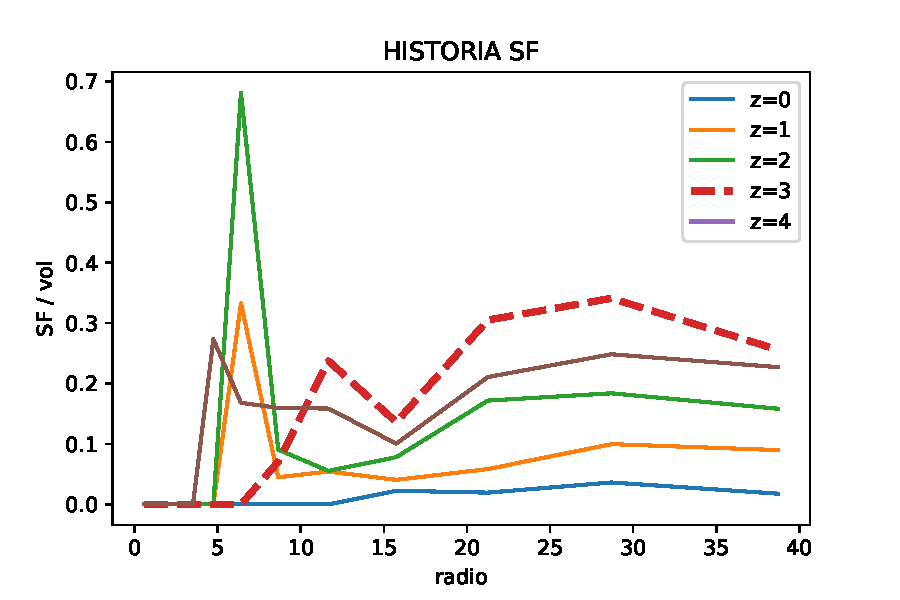
\includegraphics[width=10cm]{Figures/RSF_history.pdf}
\decoRule
\caption[RSF hsitory]{perfil diferencial de formacion estelar a diferentes redshift}
\label{fig:Electron}
\end{figure}

\begin{figure}[h]
\centering
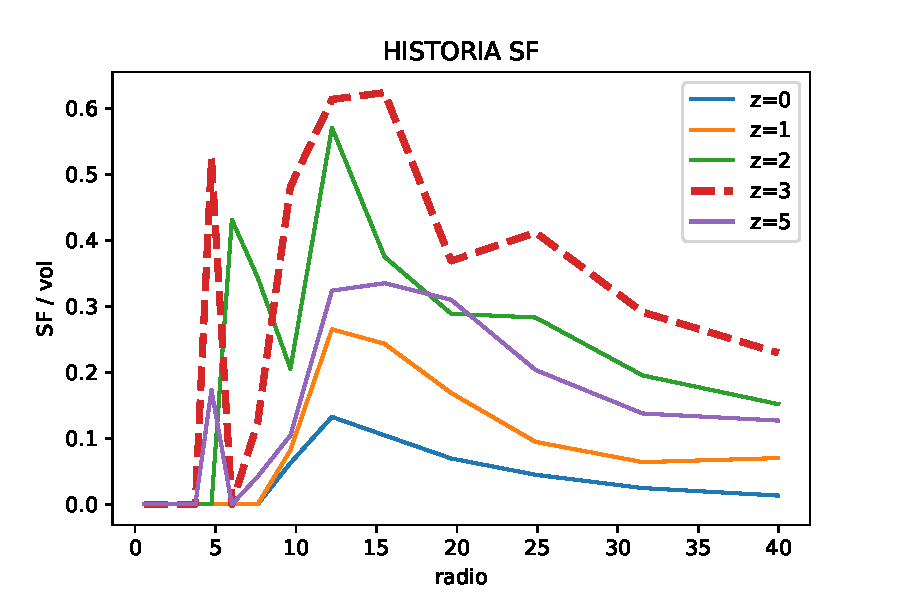
\includegraphics[width=10cm]{Figures/SSF_history.pdf}
\decoRule
\caption[SSF hsitory]{perfil diferencial de formacion estelar a diferentes redshift}
\label{fig:Electron}
\end{figure}

\begin{figure}[h]
\centering
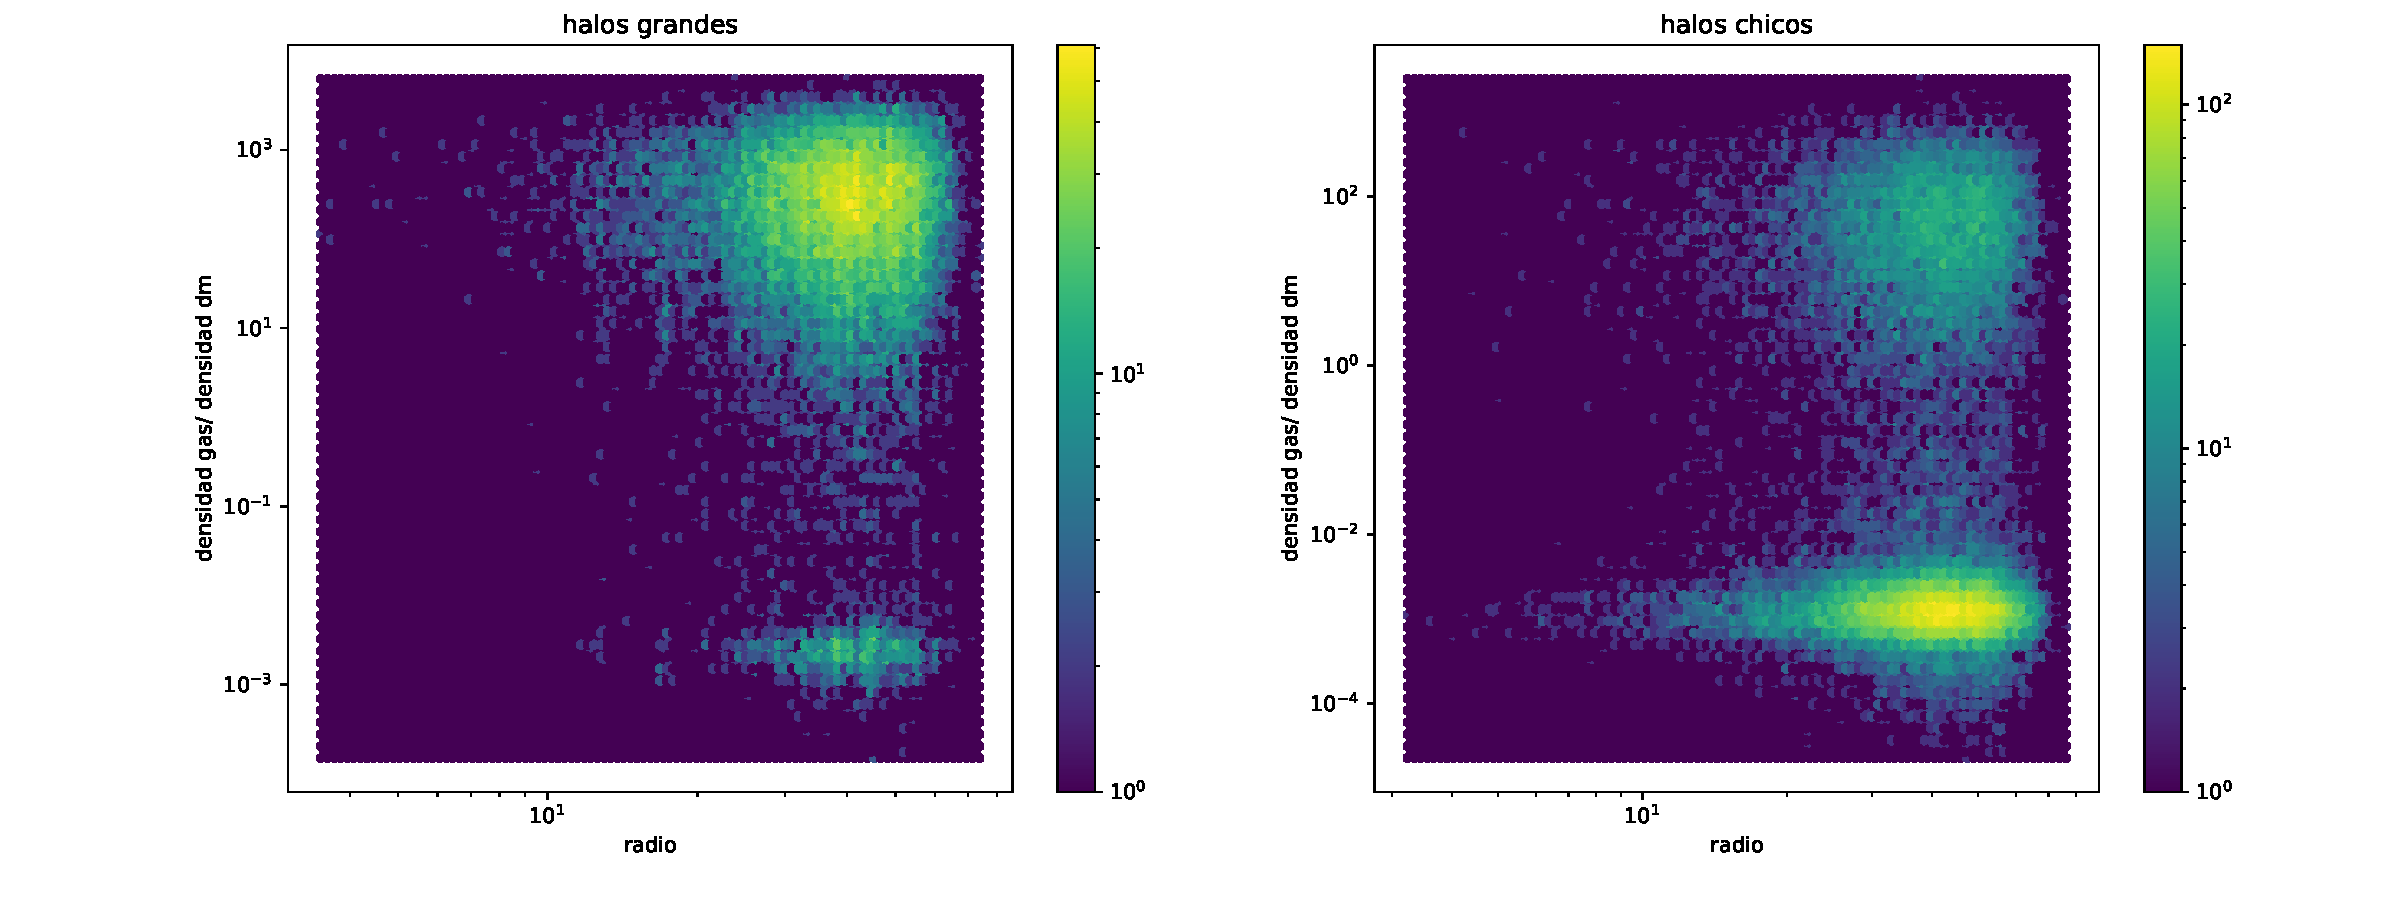
\includegraphics[width=18cm]{Figures/R_sctFRACC1.pdf}
\decoRule
\caption[perfil del void R]{}
\label{fig:Electron}
\end{figure}

\begin{figure}[h]
\centering
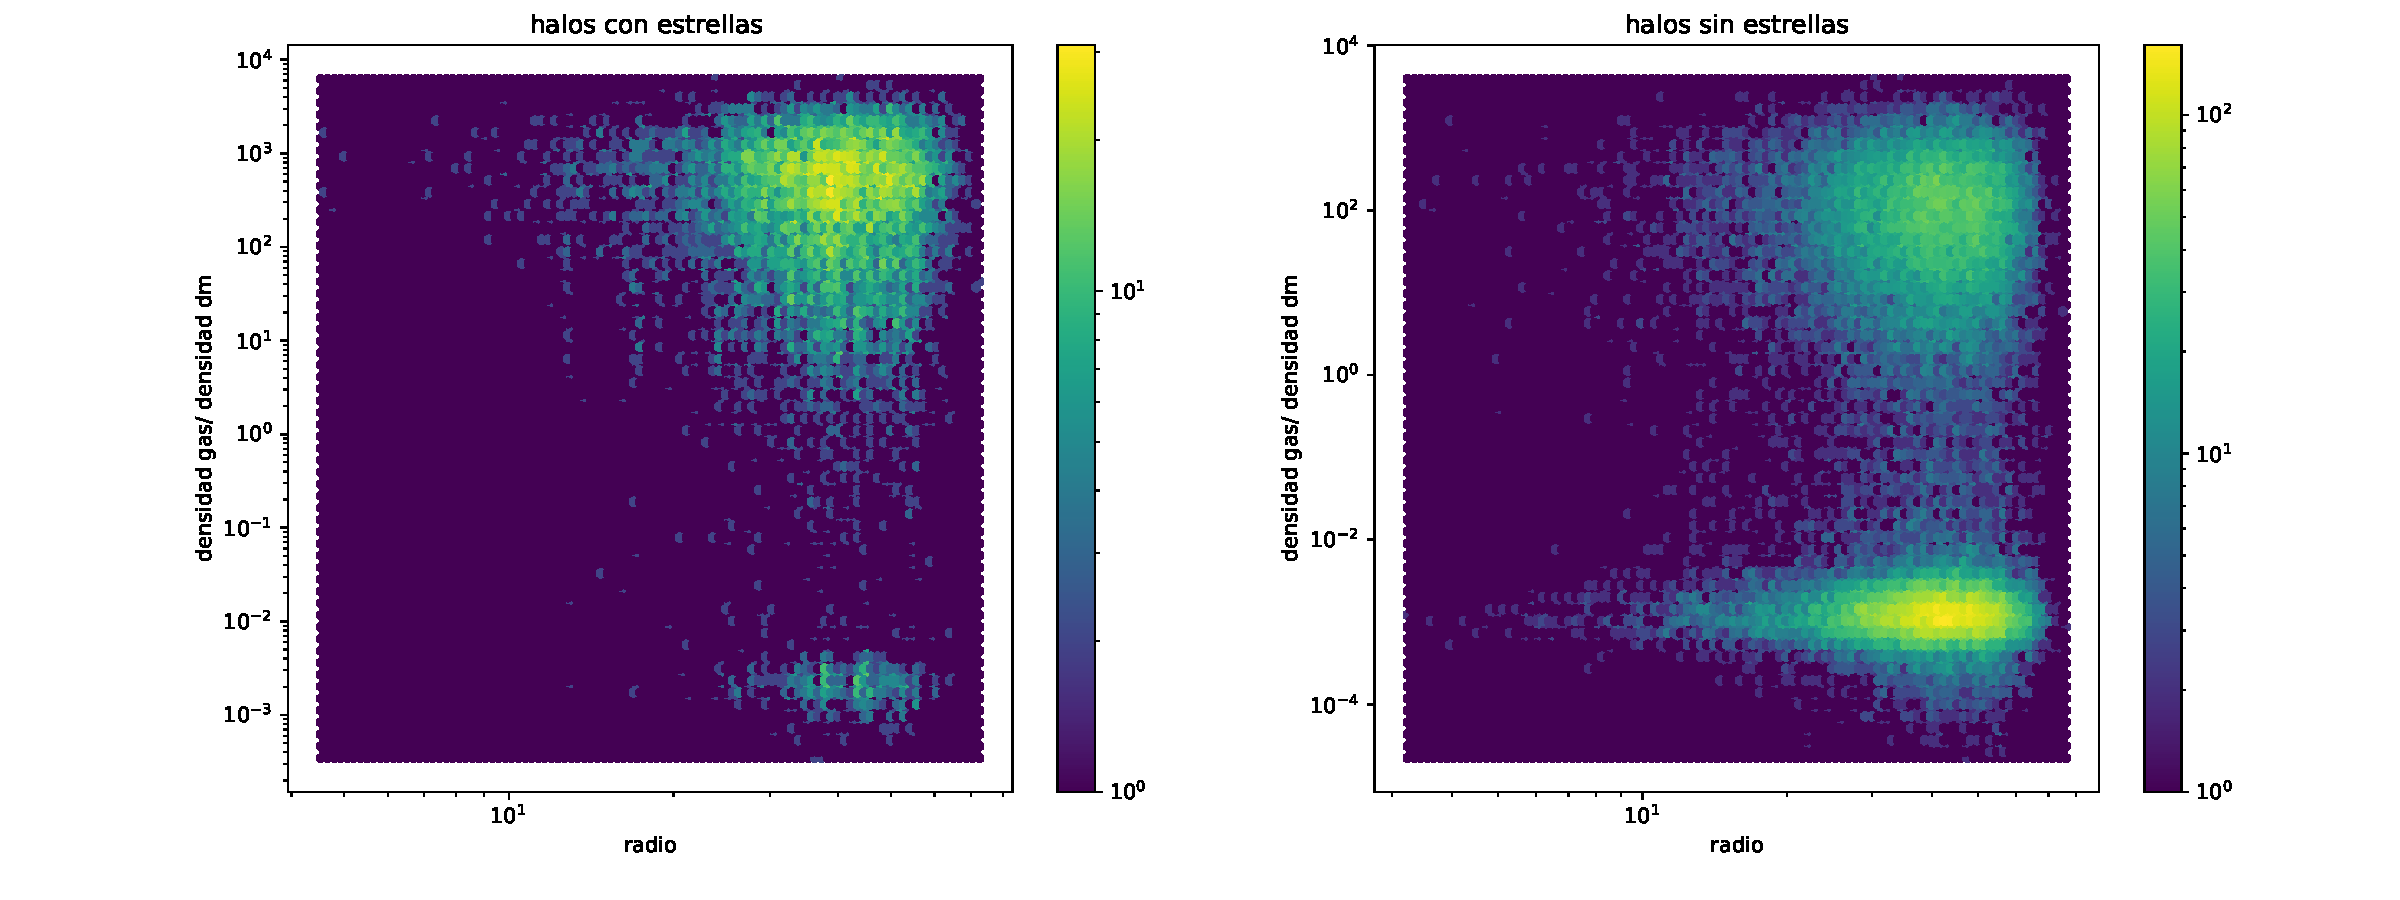
\includegraphics[width=18cm]{Figures/R_sctFRACC2.pdf}
\decoRule
\caption[perfil del void R]{}
\label{fig:Electron}
\end{figure}

\begin{figure}[h]
\centering
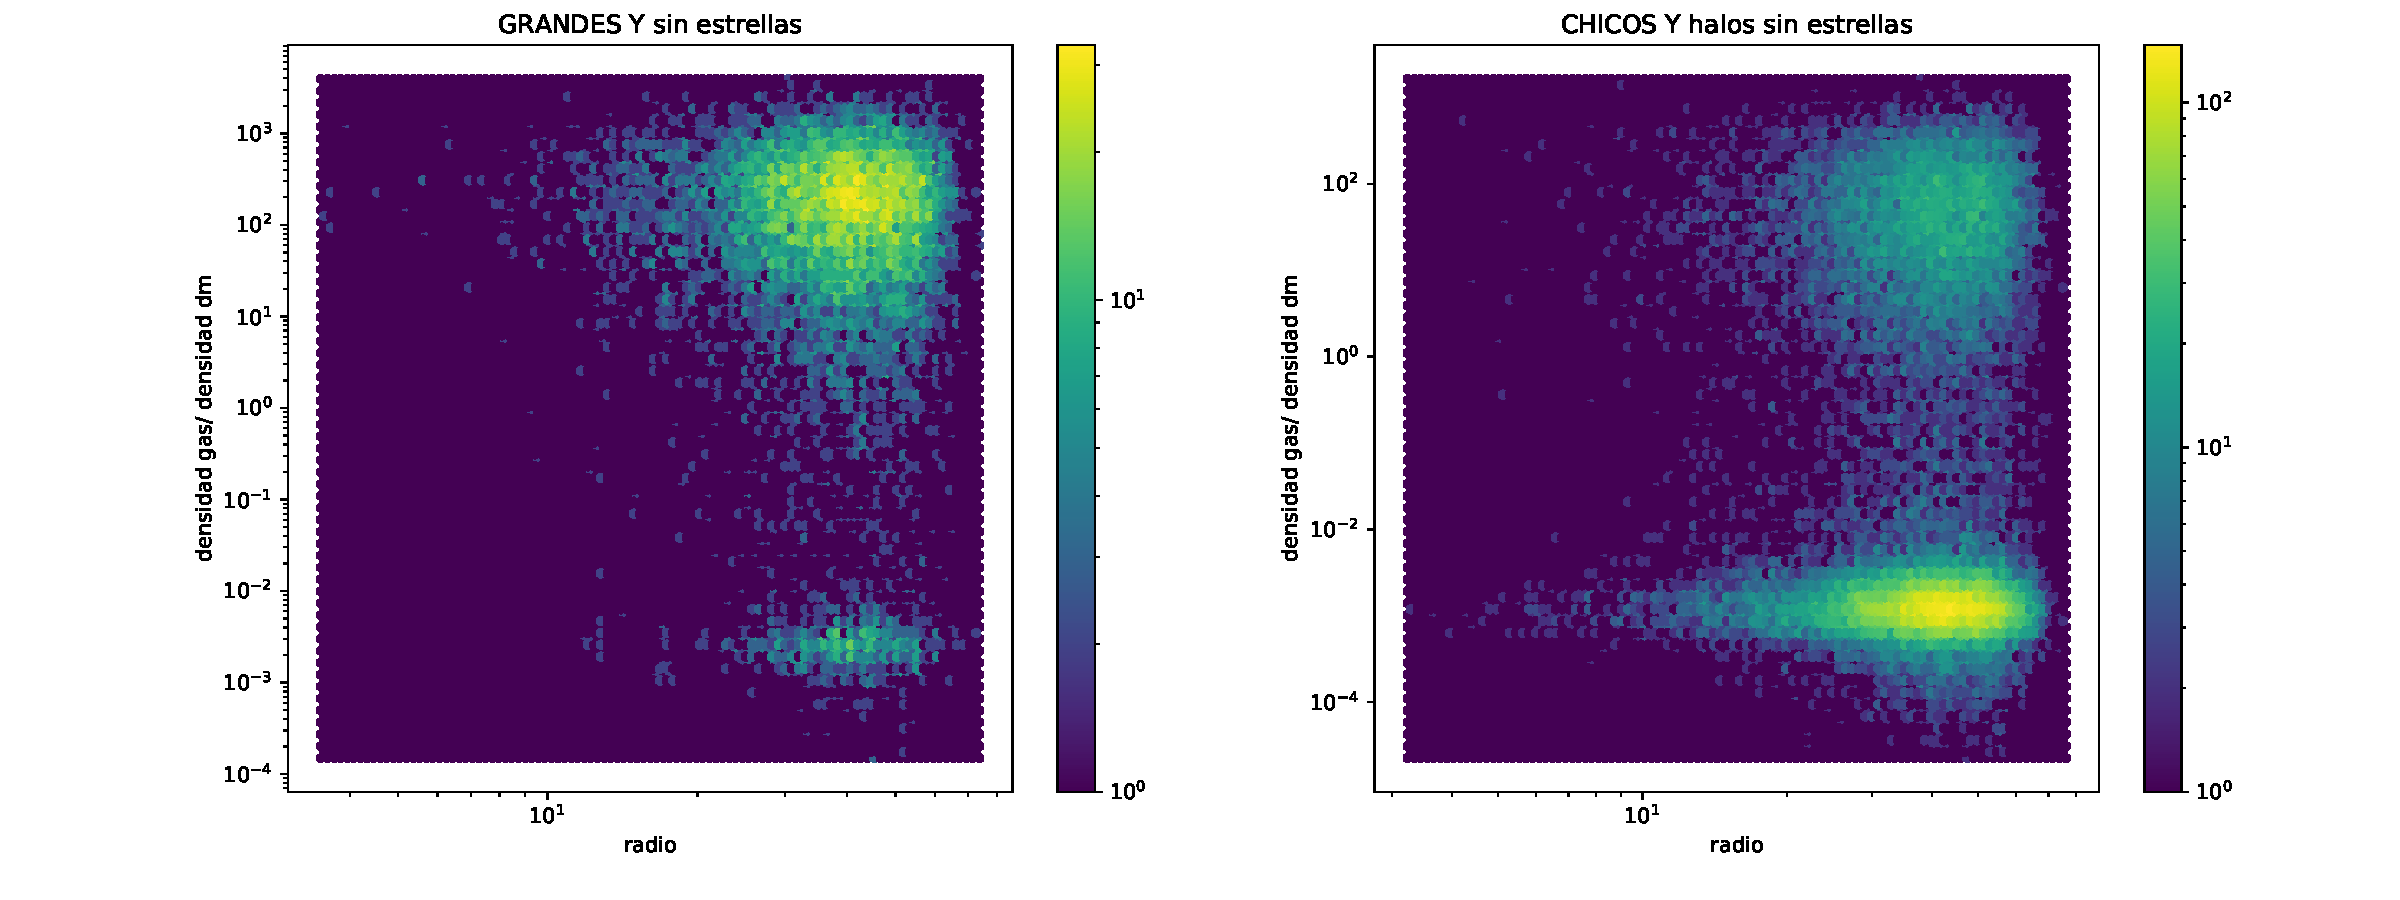
\includegraphics[width=18cm]{Figures/R_sctFRACC3.pdf}
\decoRule
\caption[perfil del void R]{}
\label{fig:Electron}
\end{figure}

\begin{figure}[h]
\centering
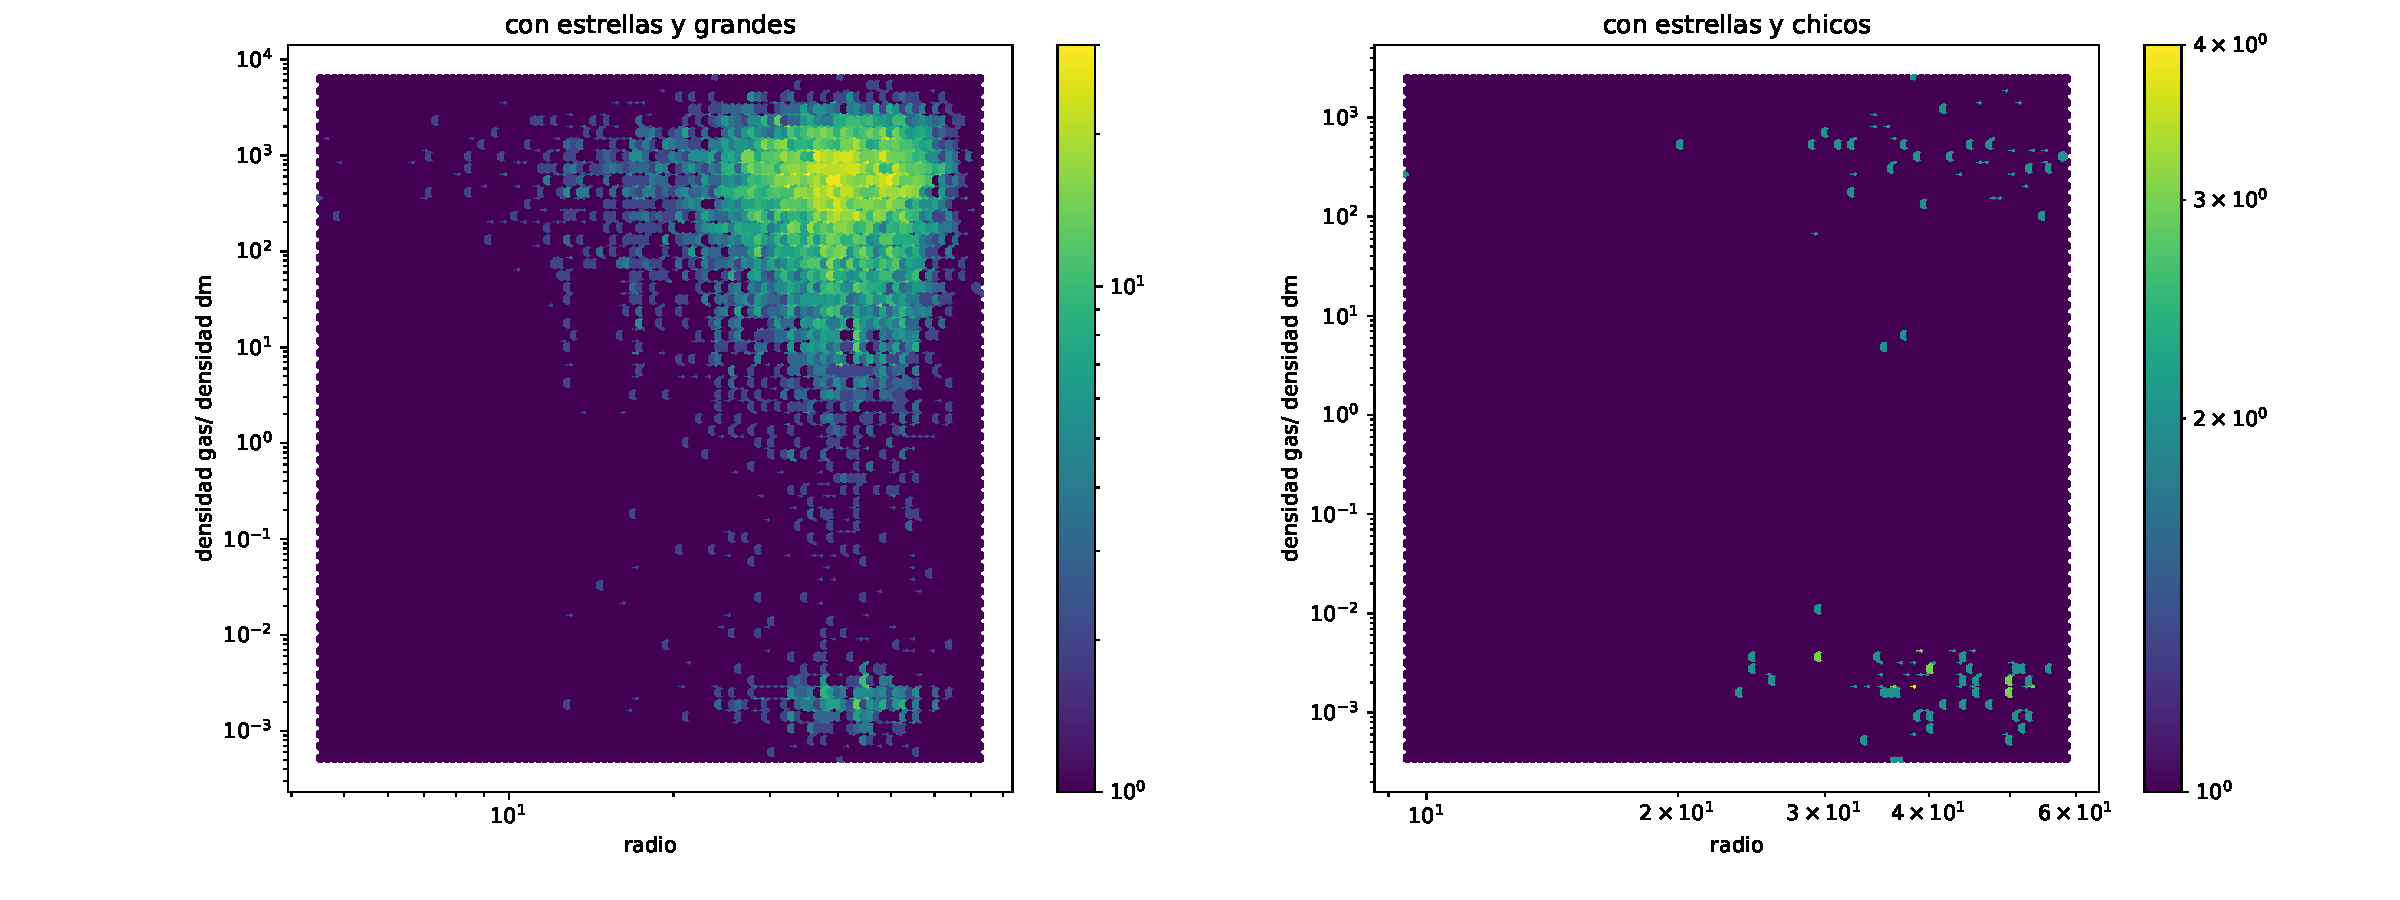
\includegraphics[width=18cm]{Figures/R_sctFRACC4.pdf}
\decoRule
\caption[perfil del void R]{}
\label{fig:Electron}
\end{figure}


\begin{figure}[h]
\centering
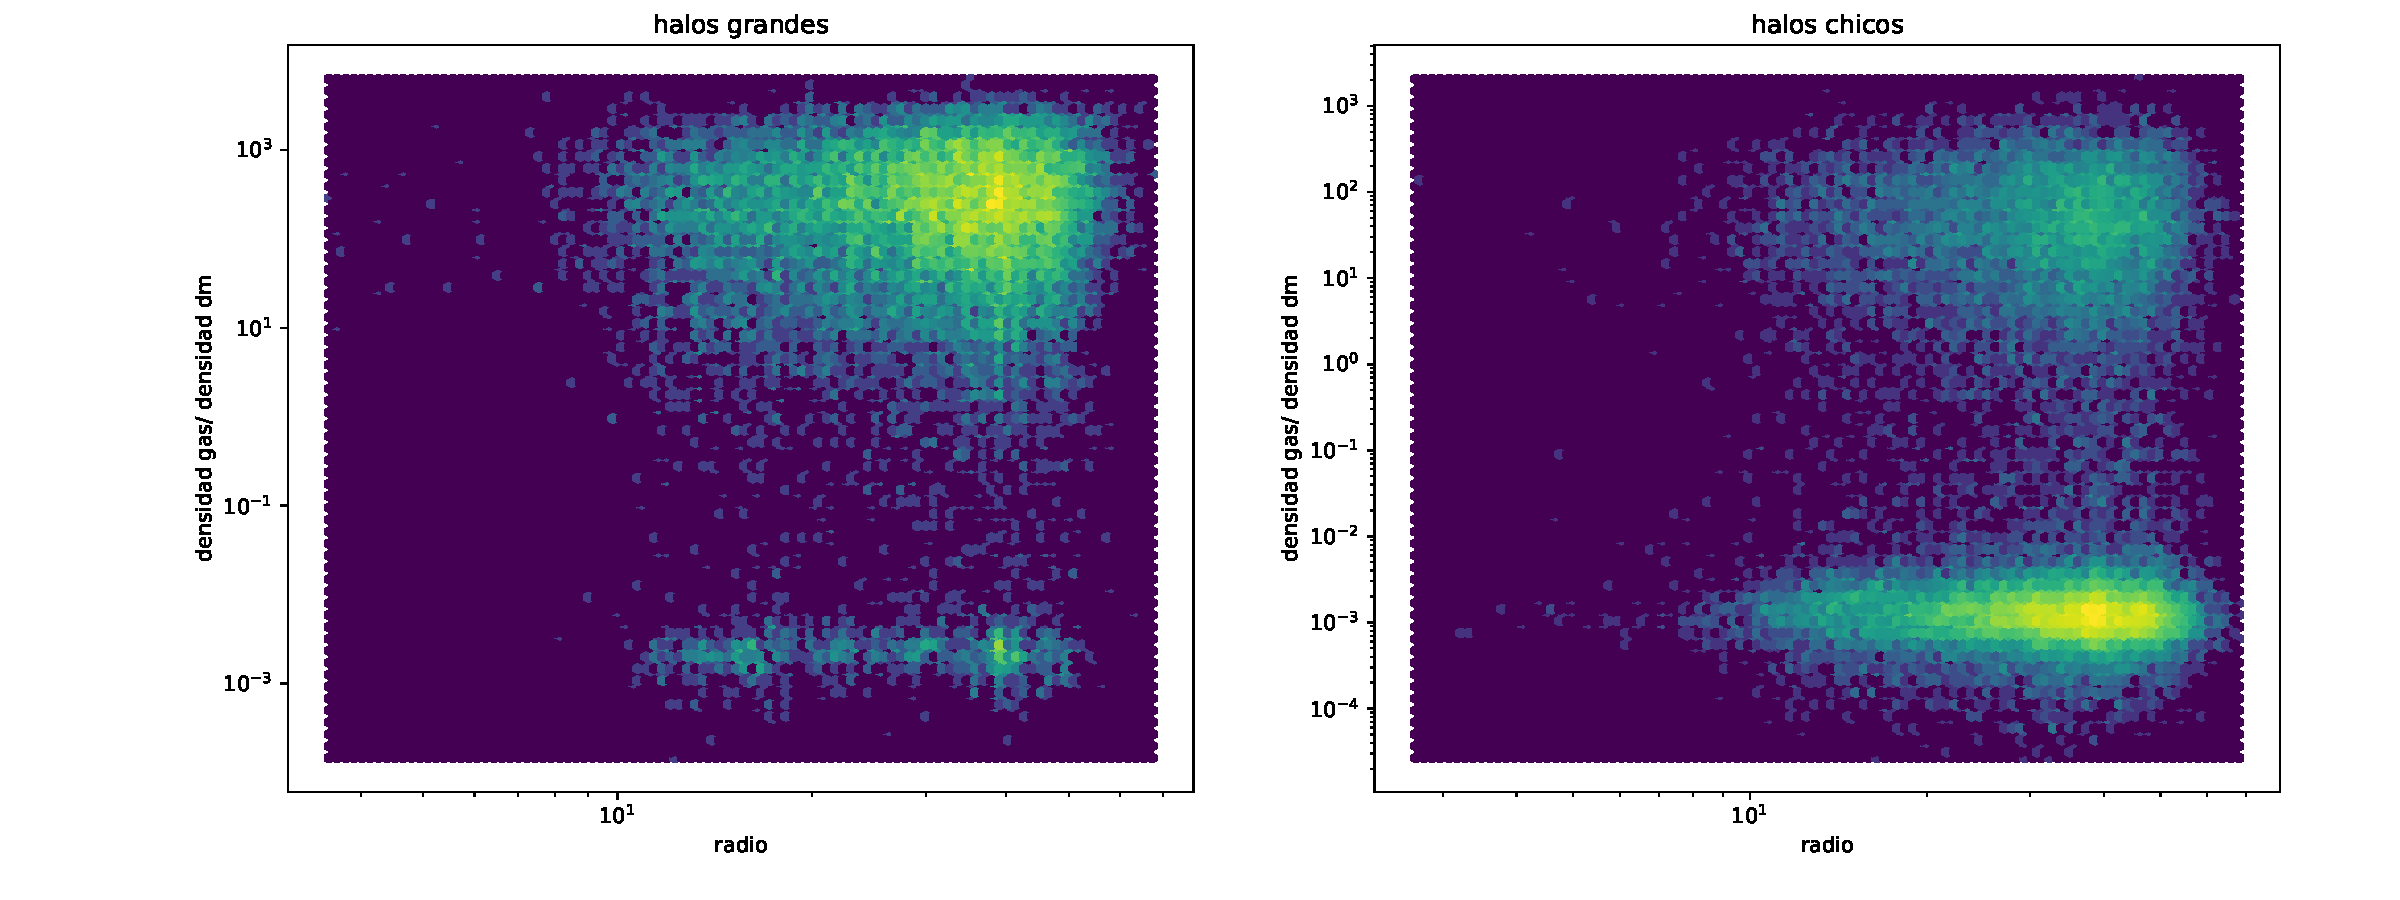
\includegraphics[width=18cm]{Figures/S_sctFRACC1.pdf}
\decoRule
\caption[perfil del void R]{}
\label{fig:Electron}
\end{figure}
\begin{figure}[h]
\centering
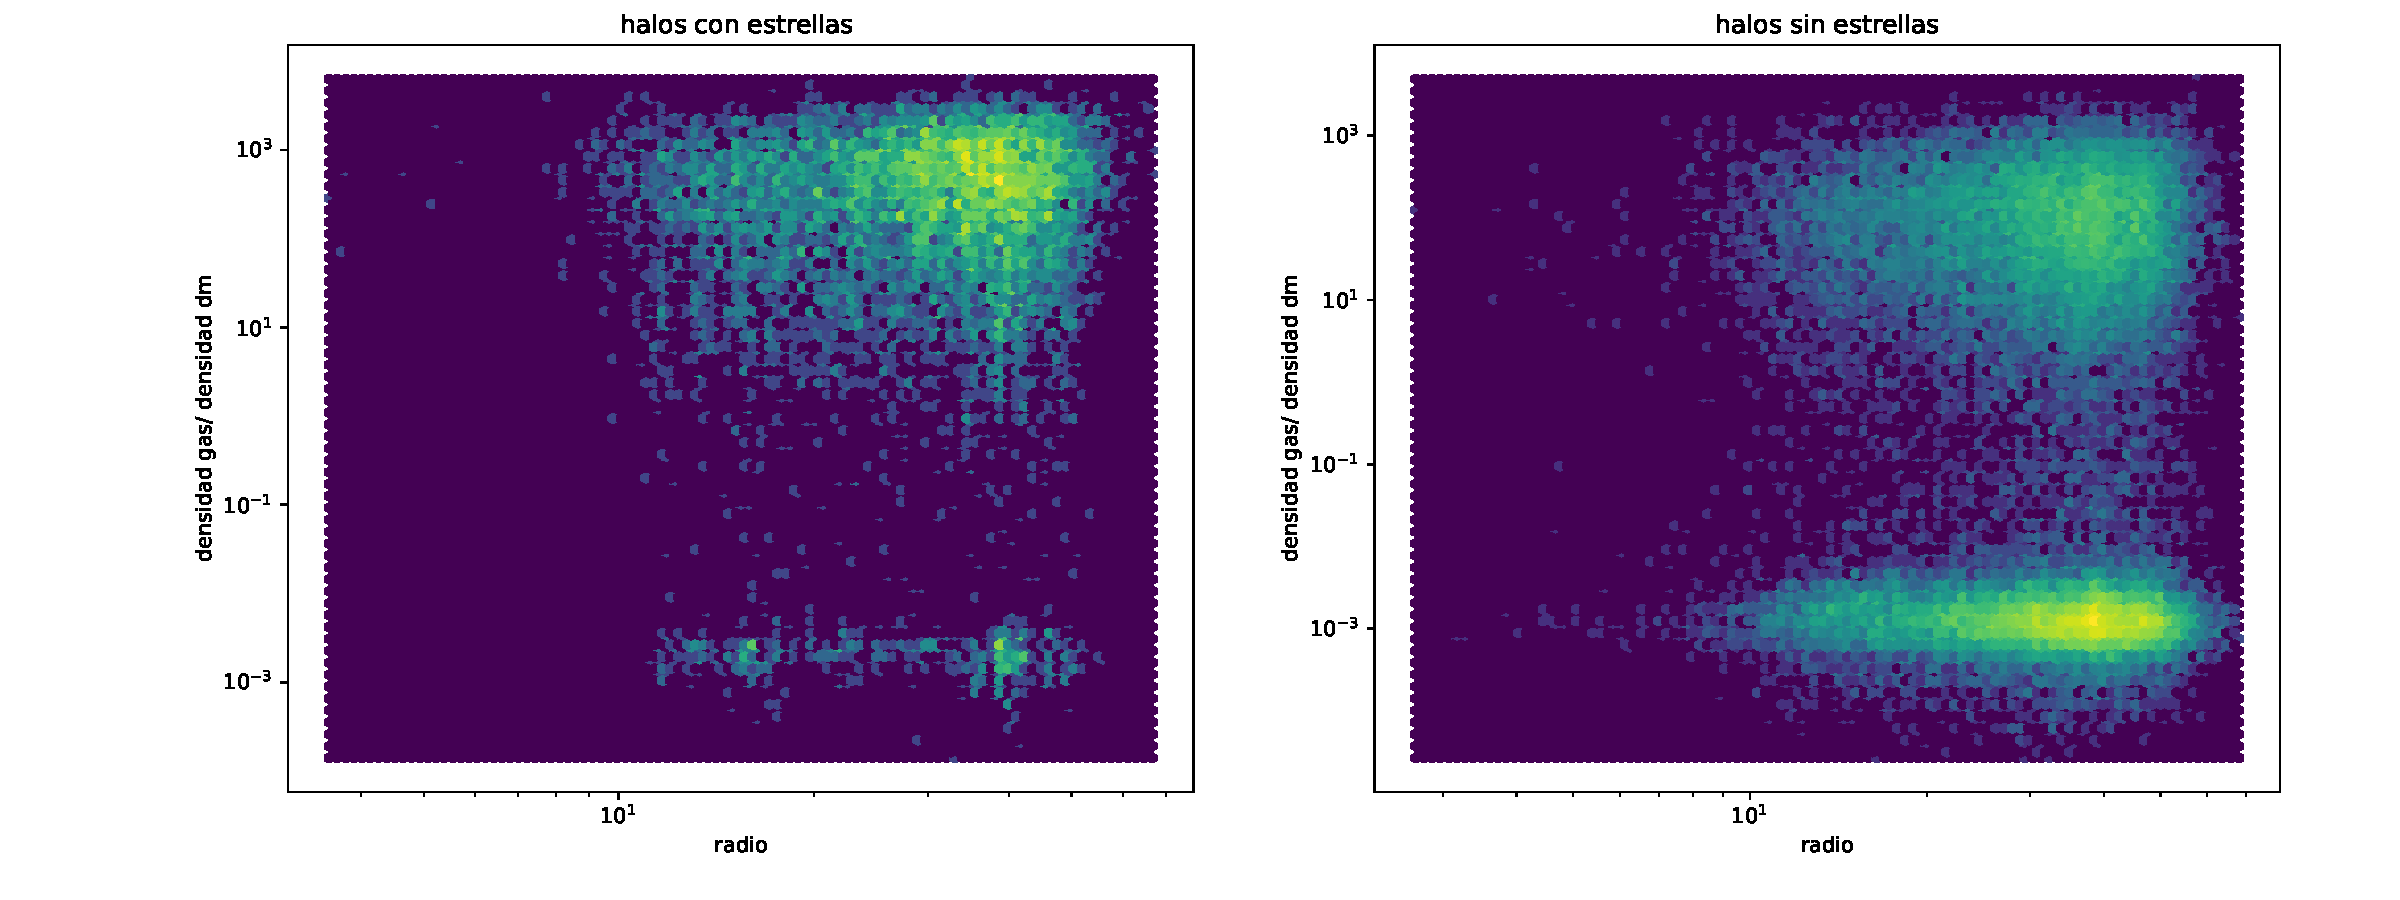
\includegraphics[width=18cm]{Figures/S_sctFRACC2.pdf}
\decoRule
\caption[perfil del void R]{}
\label{fig:Electron}
\end{figure}
\begin{figure}[h]
\centering
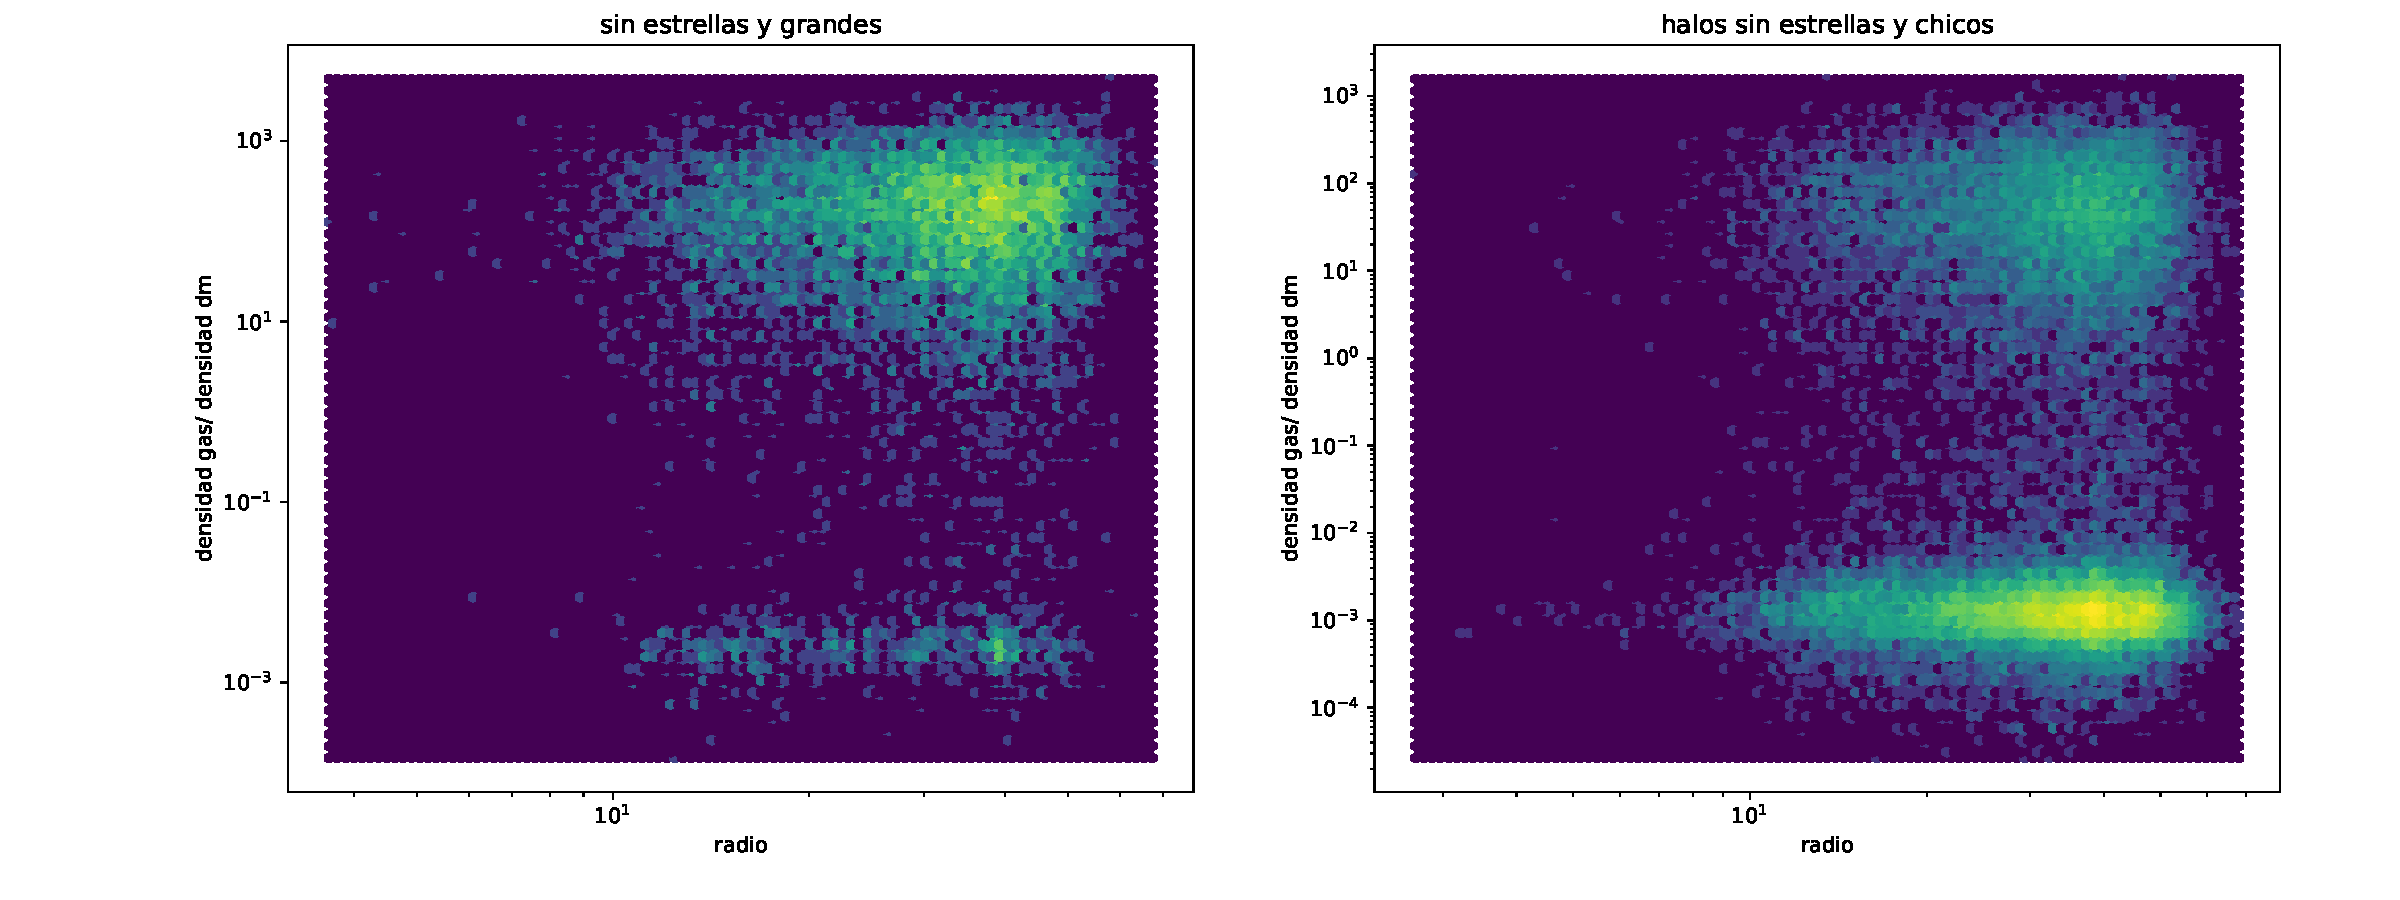
\includegraphics[width=18cm]{Figures/S_sctFRACC3.pdf}
\decoRule
\caption[perfil del void R]{}
\label{fig:Electron}
\end{figure}
\begin{figure}[h]
\centering
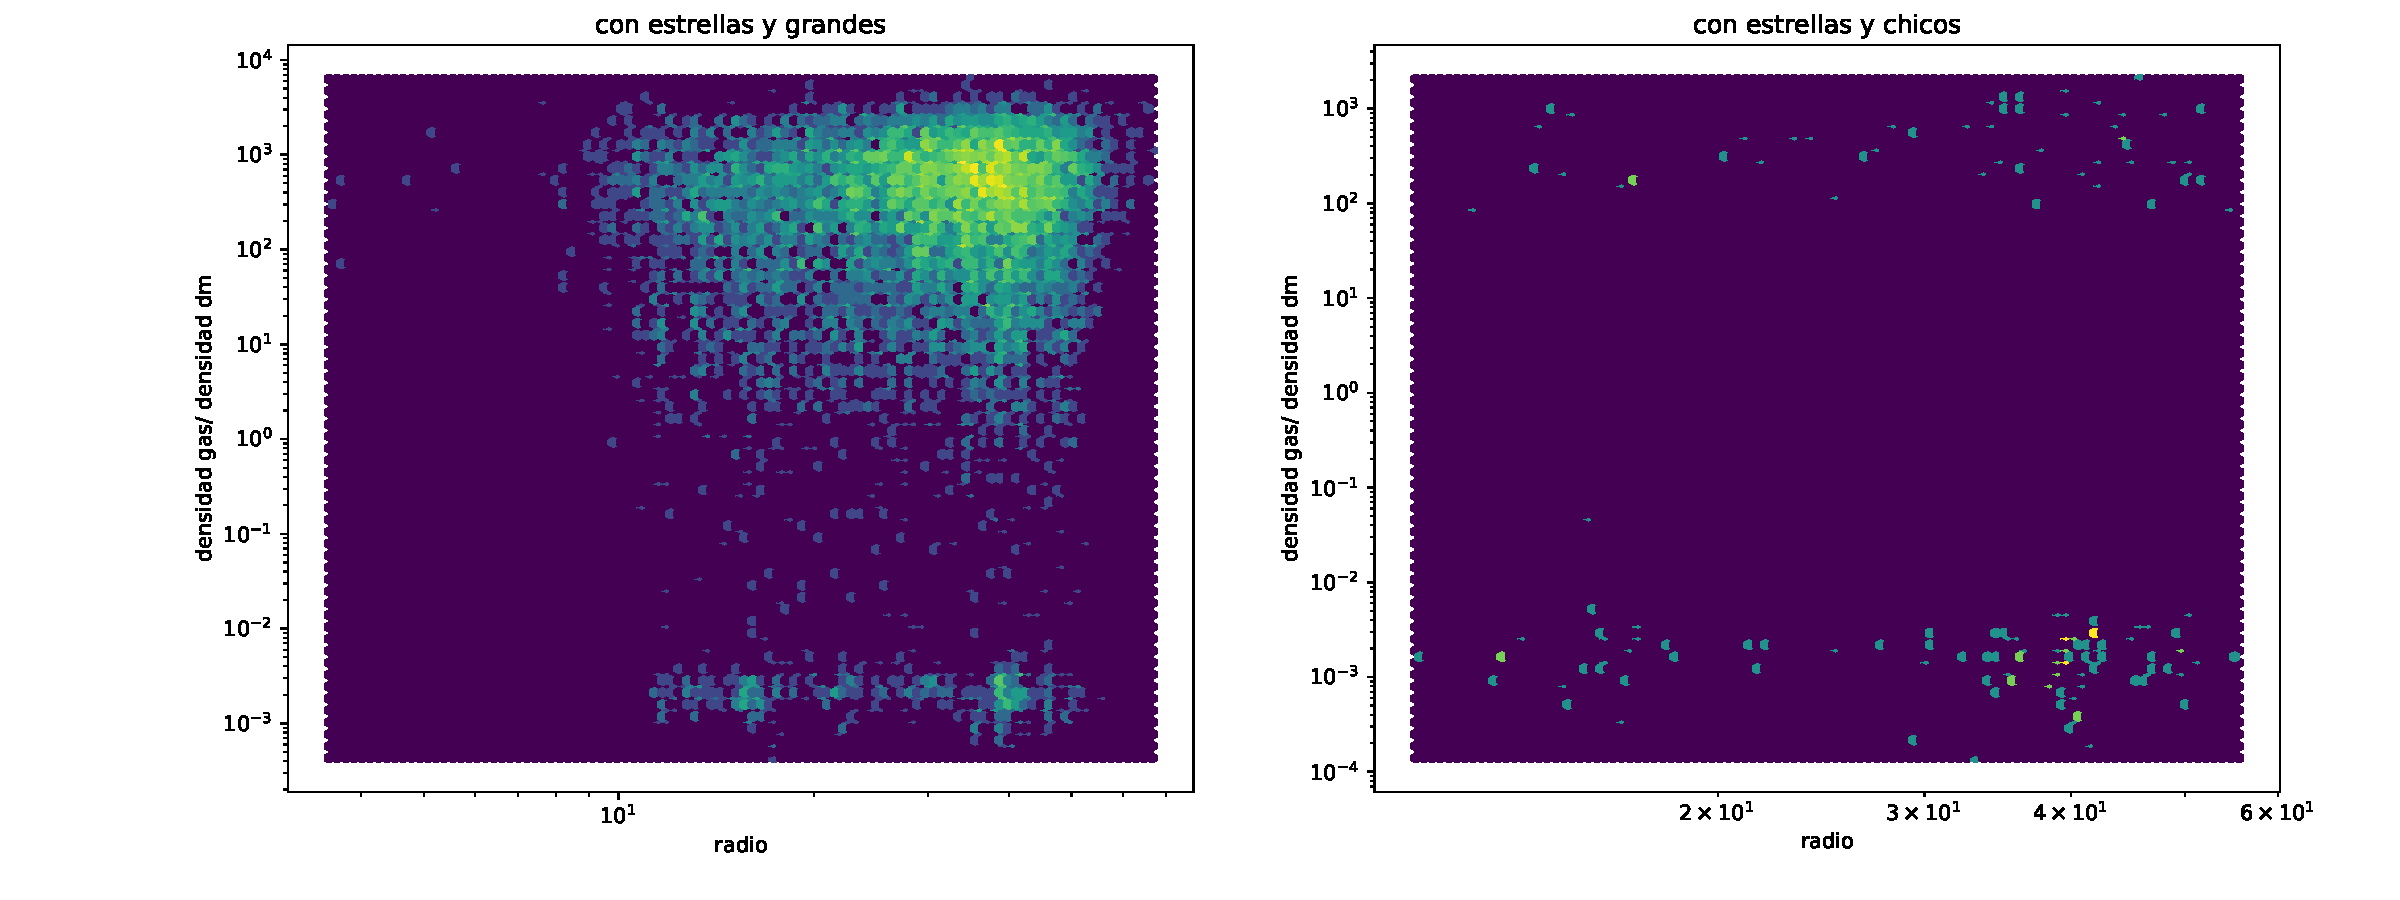
\includegraphics[width=18cm]{Figures/S_sctFRACC4.pdf}
\decoRule
\caption[perfil del void R]{}
\label{fig:Electron}
\end{figure}



\begin{figure}[h]
\centering
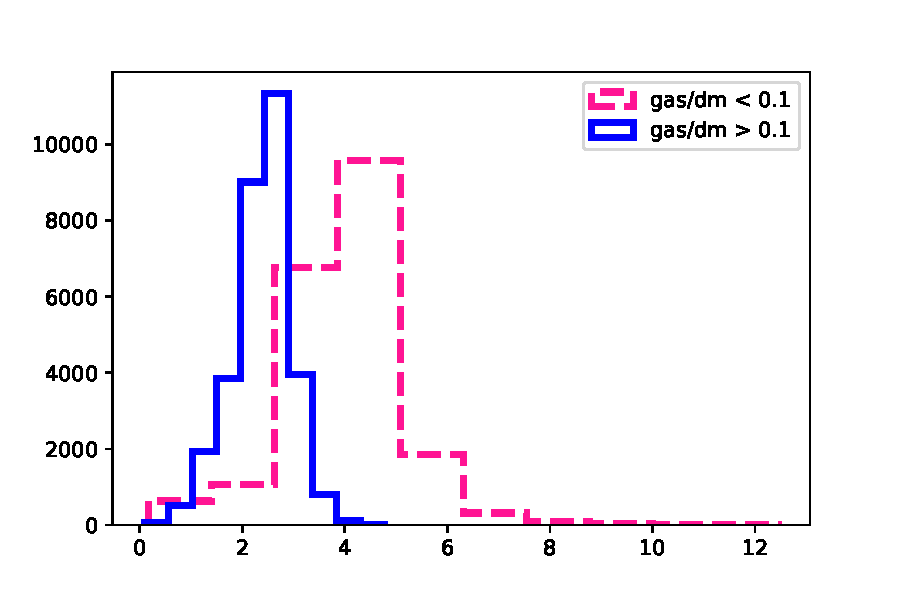
\includegraphics[width=10cm]{Figures/S_hsml.pdf}
\decoRule
\caption[asd]{VOID S distribucion para los maximo hsml/radio virial }
\label{fig:Electron}
\end{figure}

\begin{figure}[h]
\centering
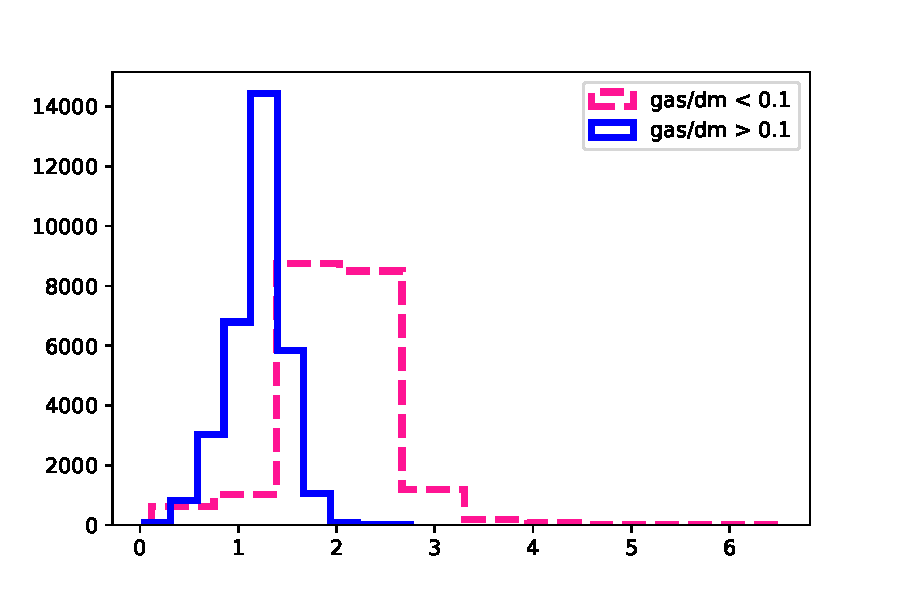
\includegraphics[width=10cm]{Figures/R_hsml.pdf}
\decoRule
\caption[asd]{VOID R distribucion para los maximo hsml/radio virial }
\label{fig:Electron}
\end{figure}

\begin{figure}[h]
\centering
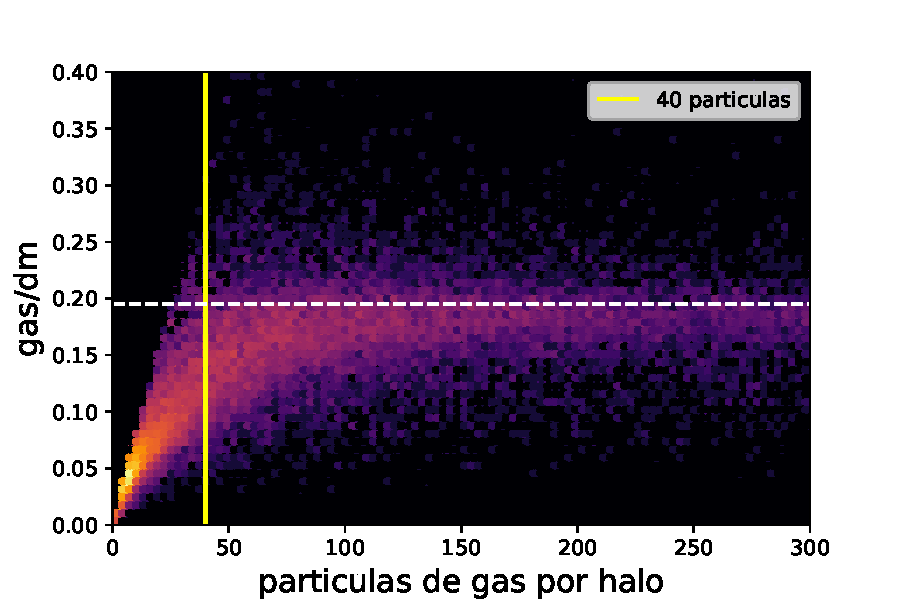
\includegraphics[width=18cm]{Figures/R_control1.pdf}
\decoRule
\caption[asd]{VOID R distribucion para los maximo hsml/radio virial }
\label{fig:Electron}
\end{figure}

\begin{figure}[h]
\centering
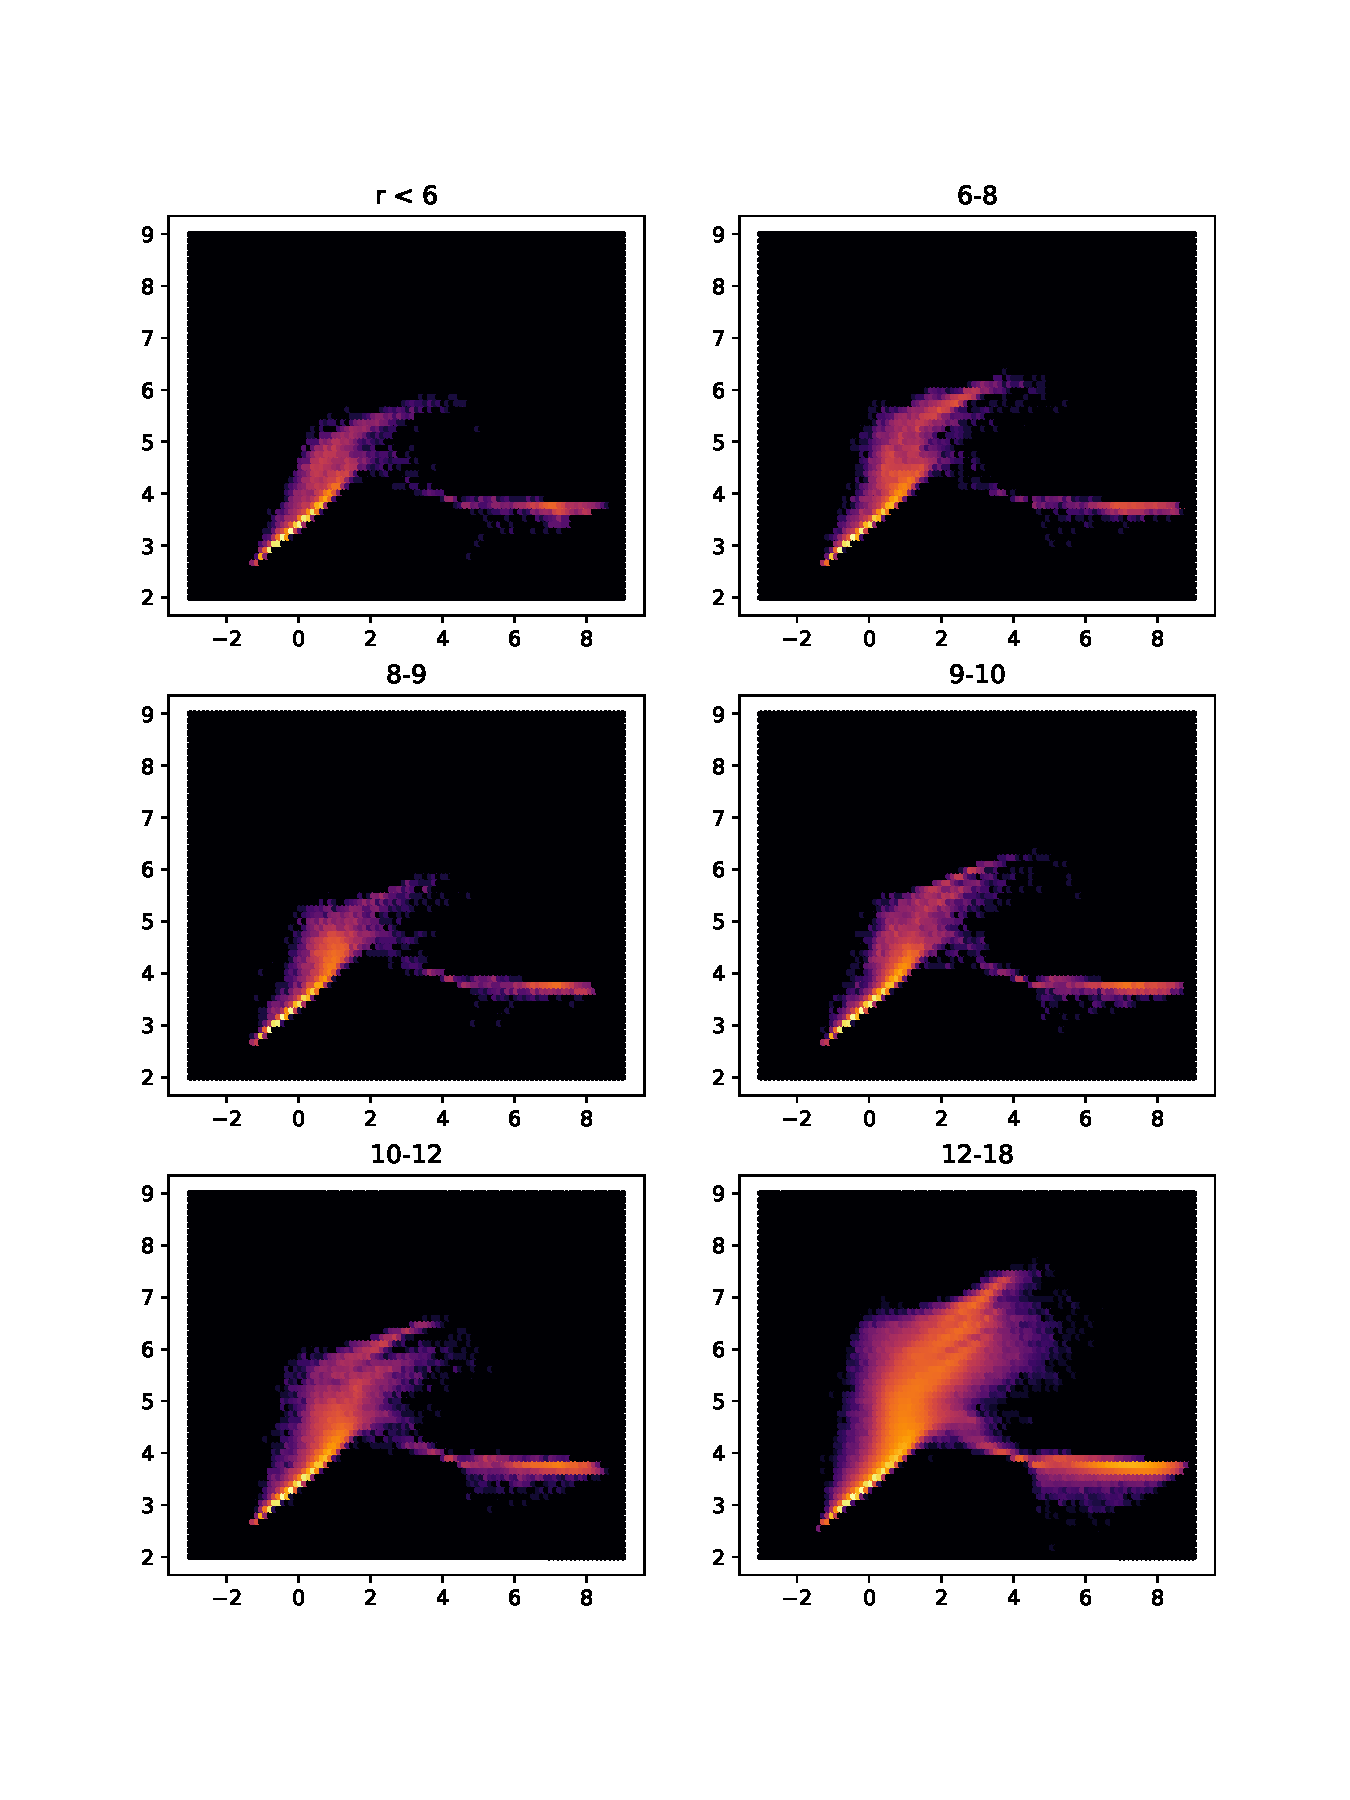
\includegraphics[width=15cm]{Figures/R1198_DF1.pdf}
\decoRule
\caption[asd]{diagramas de fase para el void R1198}
\label{fig:Electron}
\end{figure}

\begin{figure}[h]
\centering
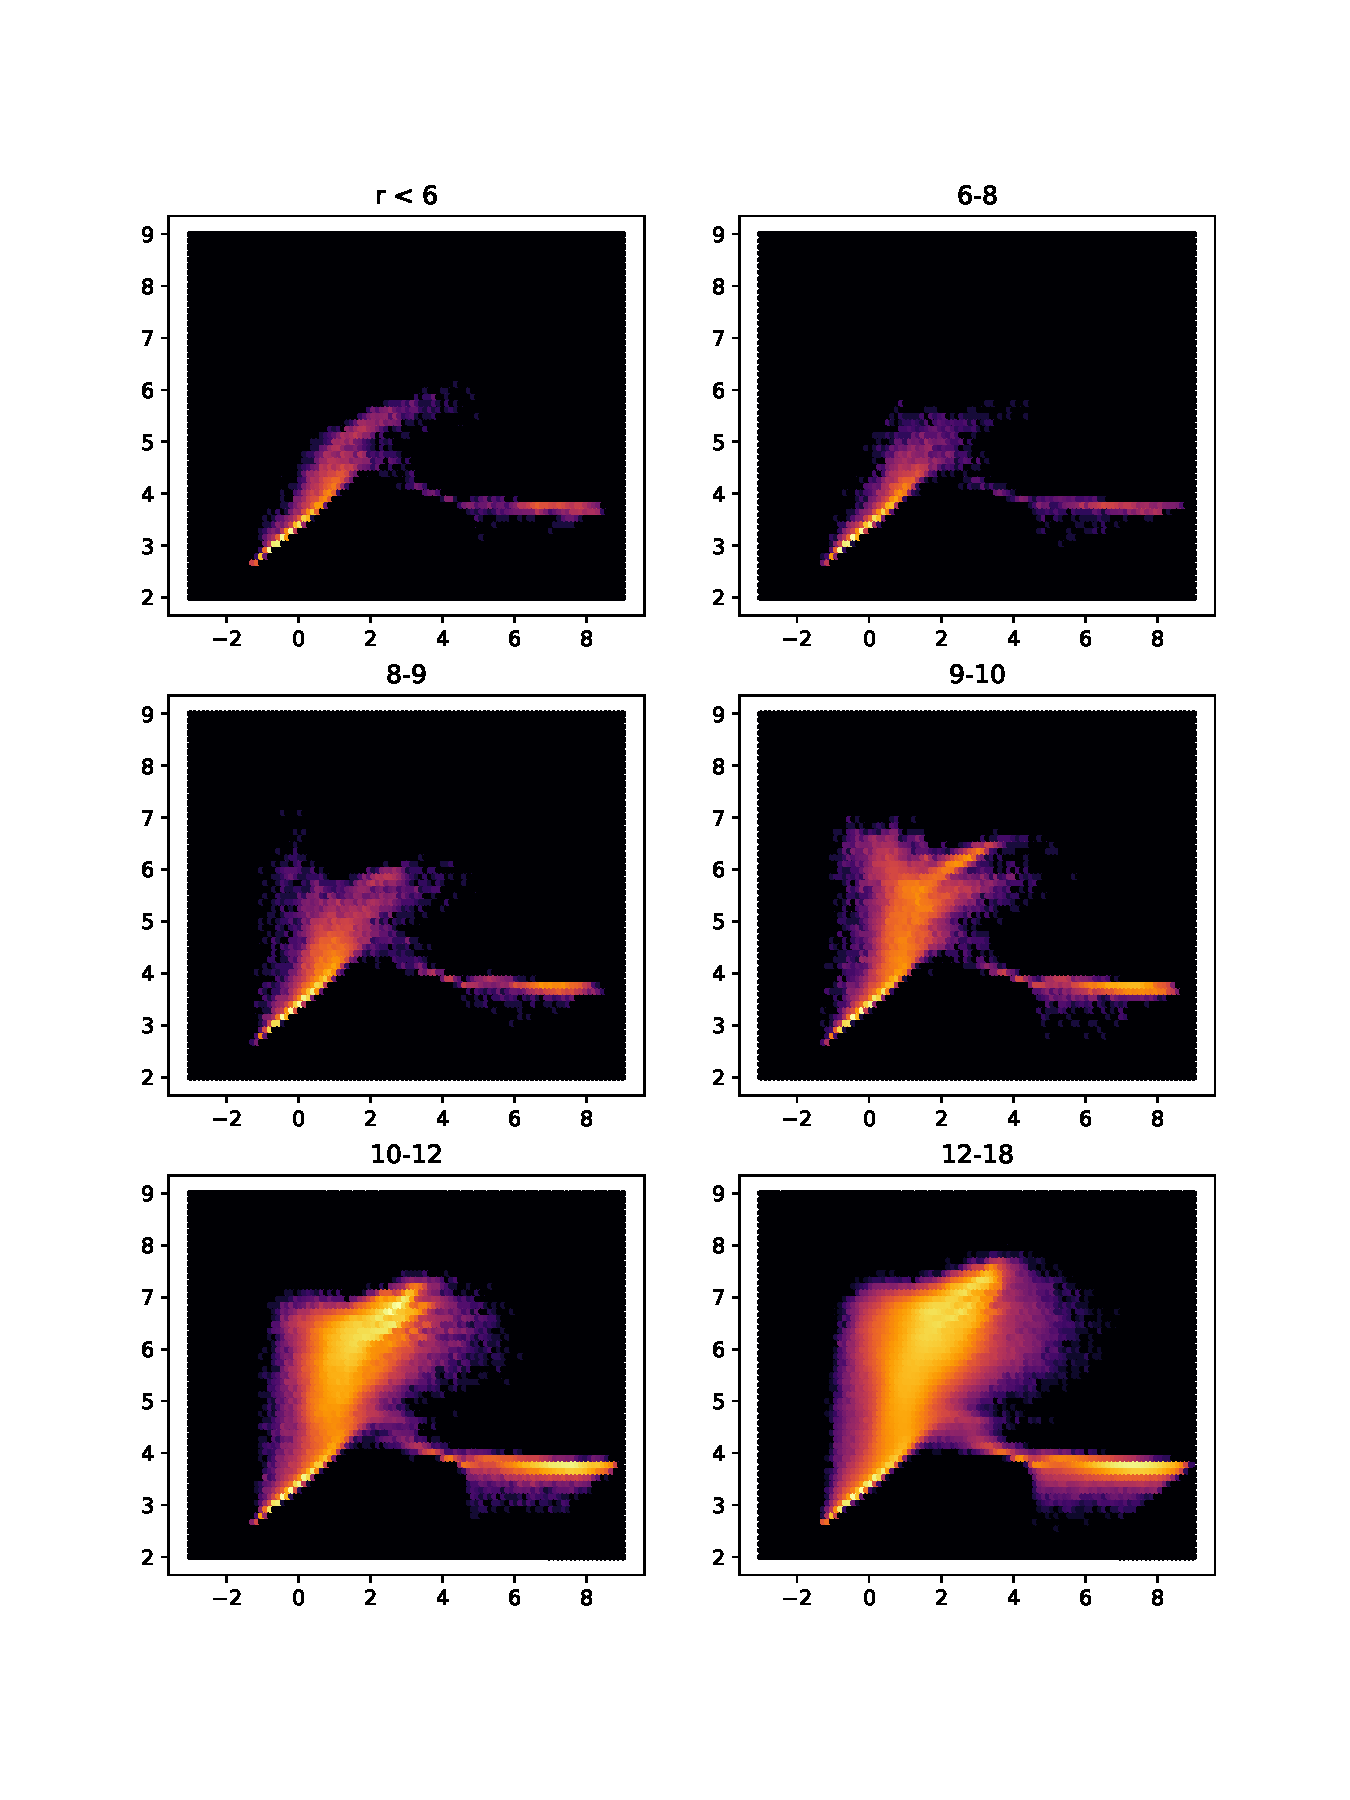
\includegraphics[width=15cm]{Figures/S1373_DF1.pdf}
\decoRule
\caption[asd]{diagramas de fase para el void S}
\label{fig:Electron}
\end{figure}

\begin{figure}[h]
\centering
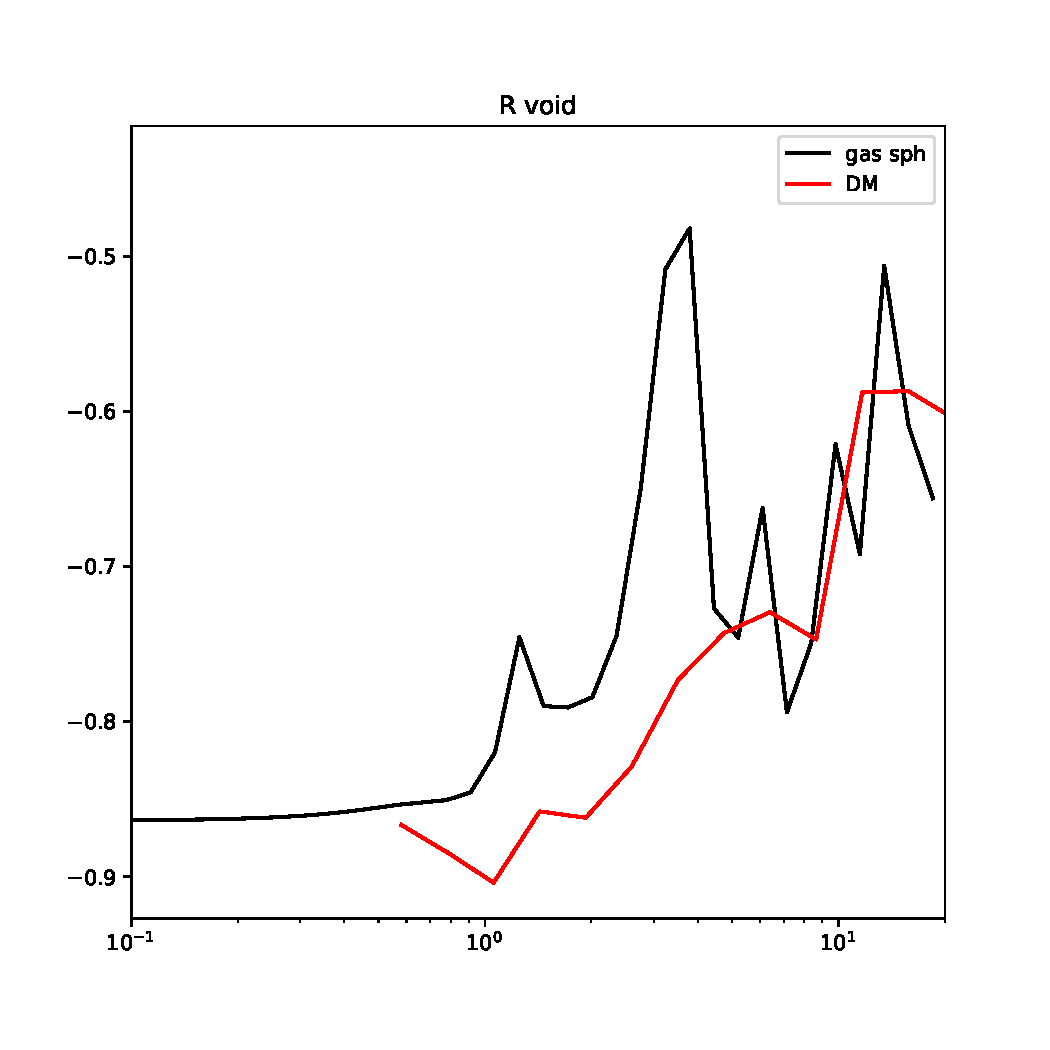
\includegraphics[width=15cm]{Figures/R1198_sph1.pdf}
\decoRule
\caption[asd]{diagramas de fase para el void S}
\label{fig:Electron}
\end{figure}

\begin{figure}[h]
\centering
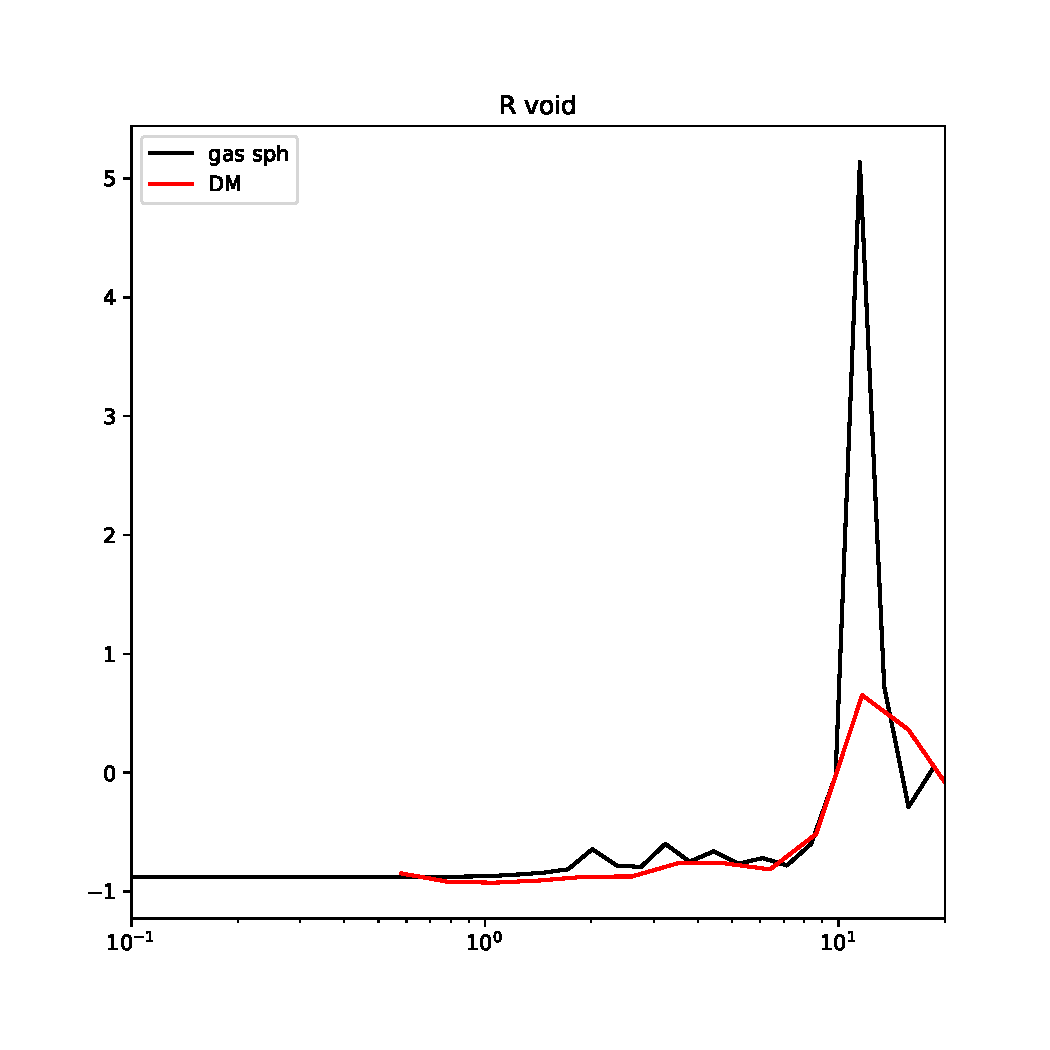
\includegraphics[width=15cm]{Figures/S1373_sph1.pdf}
\decoRule
\caption[asd]{diagramas de fase para el void S}
\label{fig:Electron}
\end{figure}

\begin{figure}[h]
\centering
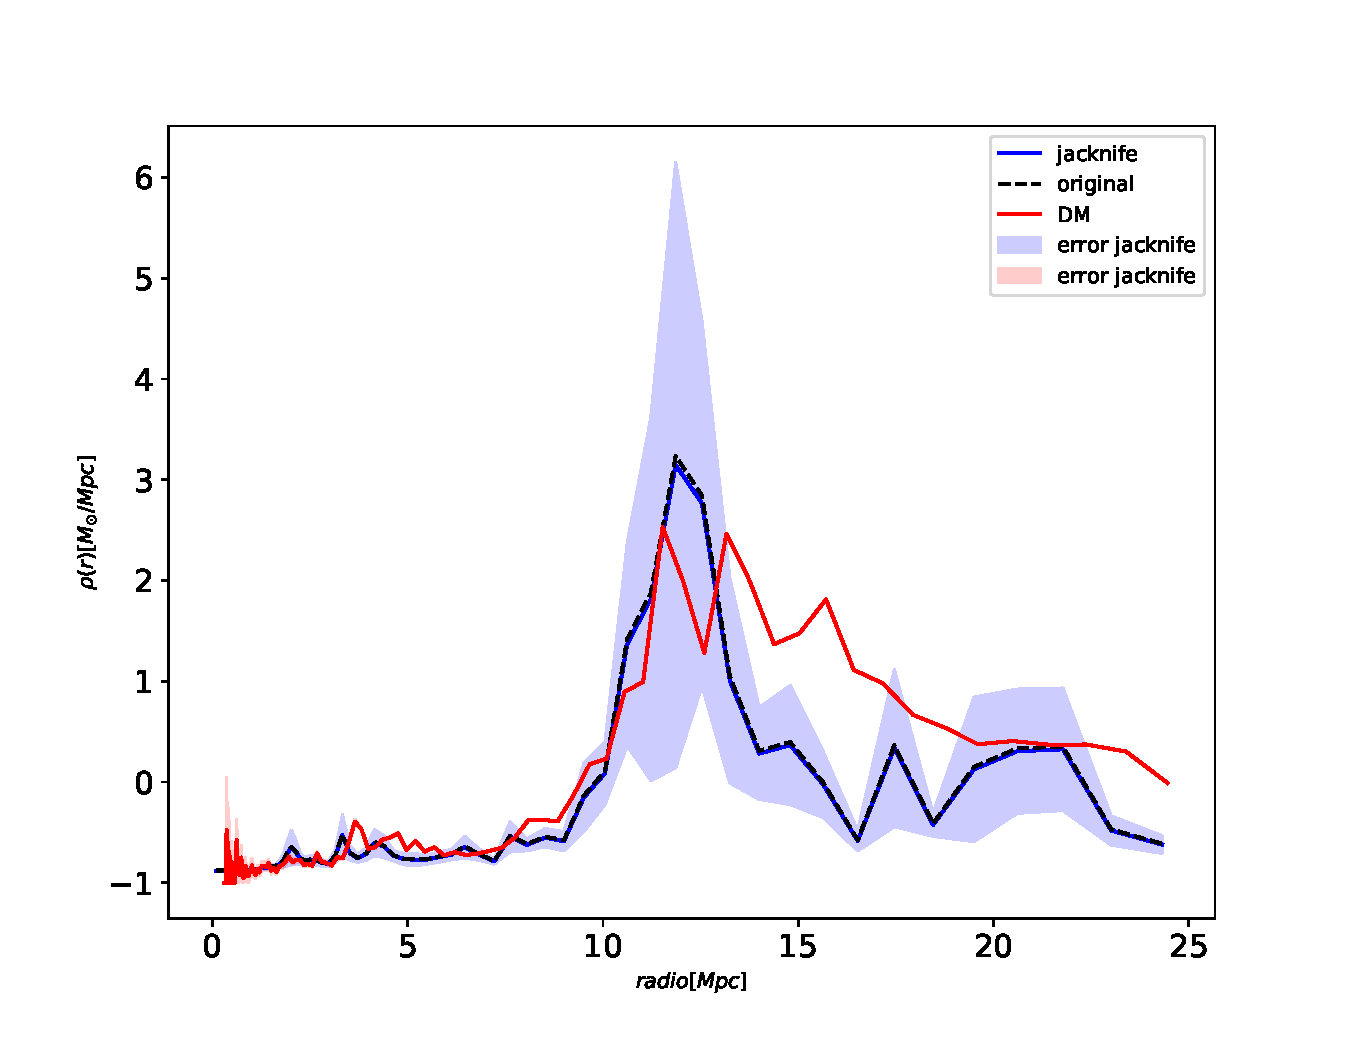
\includegraphics[width=15cm]{Figures/S1373_sph2.pdf}
\decoRule
\caption[asd]{diagramas de fase para el void S}
\label{fig:Electron}
\end{figure}

\begin{figure}[h]
\centering
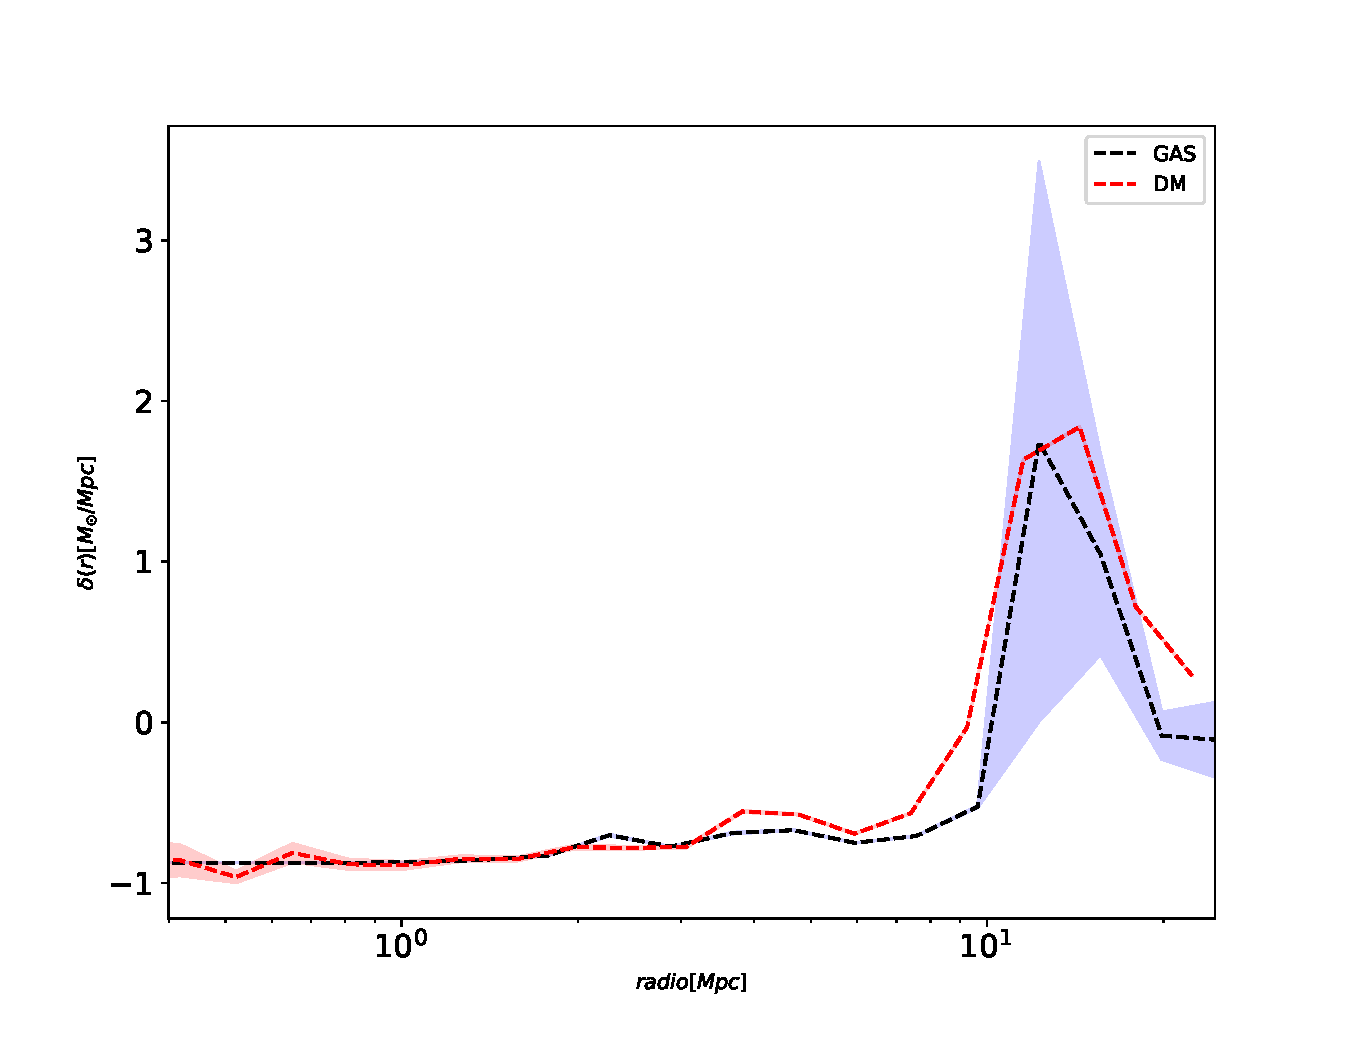
\includegraphics[width=15cm]{Figures/S1373_sph3.pdf}
\decoRule
\caption[asd]{Perfil de densidad diferencial para el void S. Se promediaron 200 muestras cada 10. }
\label{fig:Electron}
\end{figure}

\begin{figure}[h]
\centering
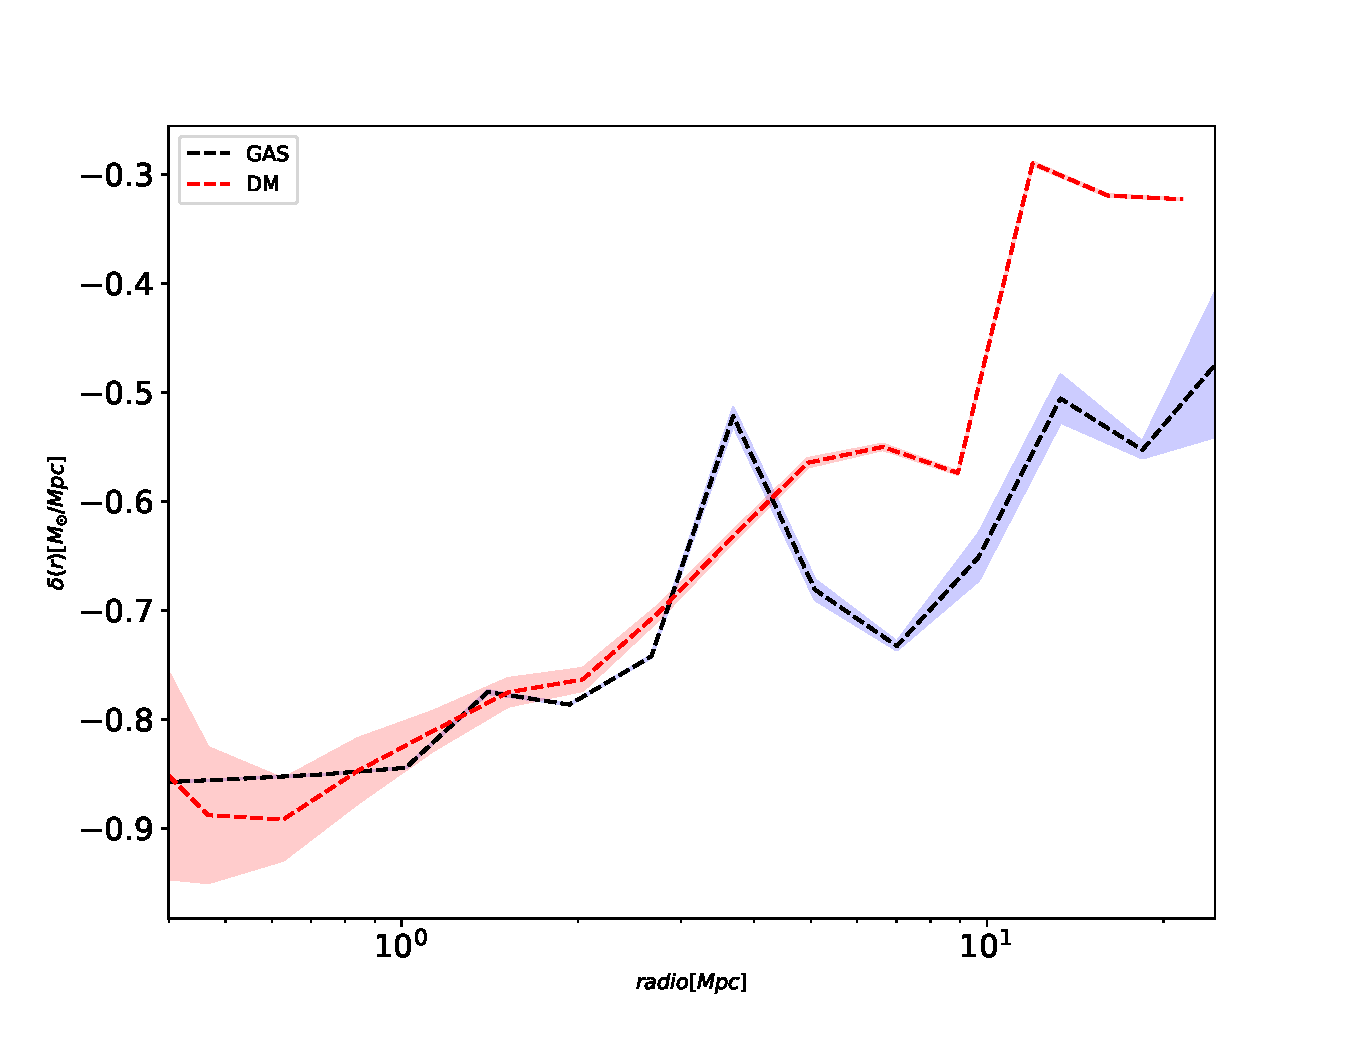
\includegraphics[width=15cm]{Figures/R1198_sph3.pdf}
\decoRule
\caption[asd]{Perfil de densidad diferencial para el void R. Se promediaron 200 muestras cada 10. }
\label{fig:Electron}
\end{figure}

\begin{figure}[h]
\centering
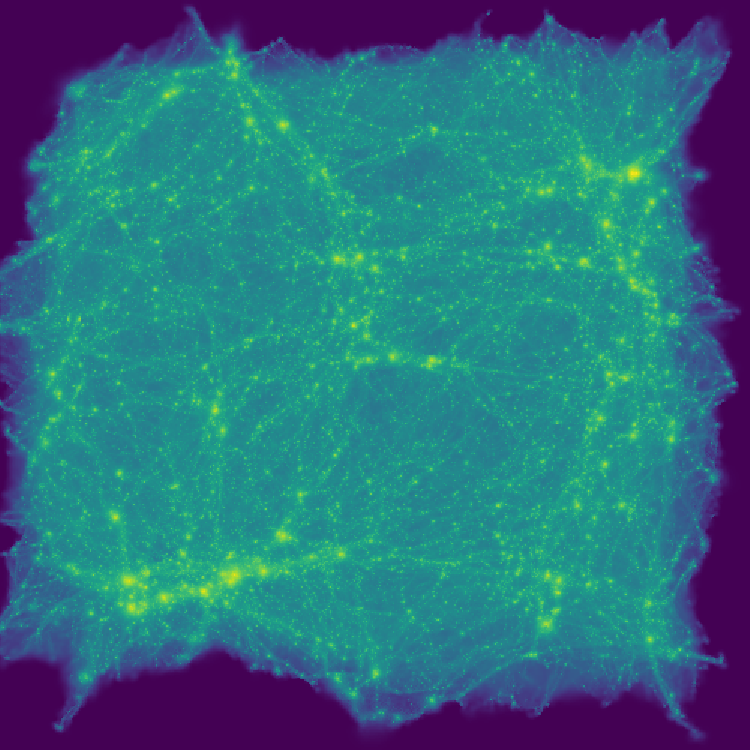
\includegraphics[width=15cm]{Figures/R1198_zoomin1.pdf}
\decoRule
\caption[asd]{resimulacion del void R }
\label{fig:Electron}
\end{figure}

\begin{figure}[h]
\centering
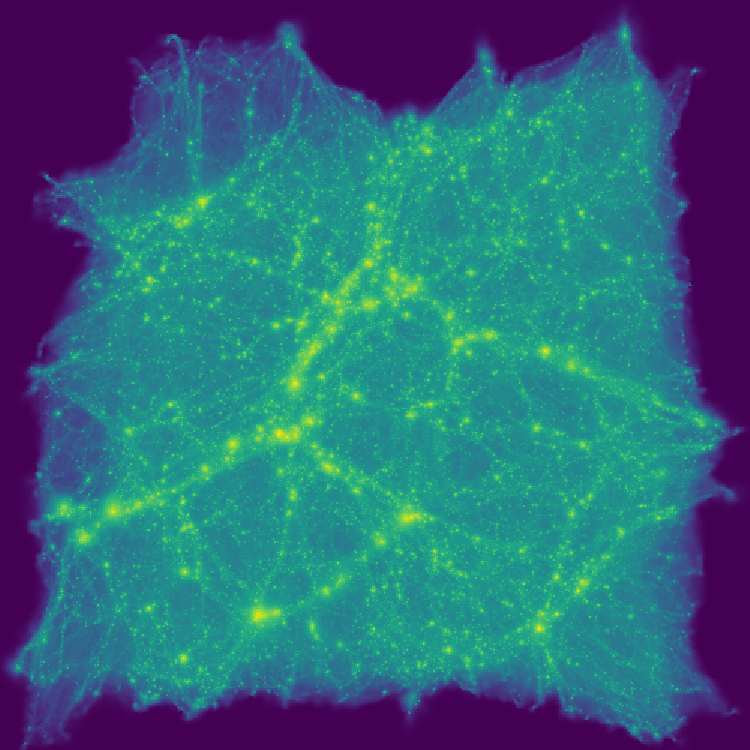
\includegraphics[width=15cm]{Figures/S1373_zoomin1.pdf}
\decoRule
\caption[asd]{resiumacion del void S }
\label{fig:Electron}
\end{figure}